\section{Method}
\label{sec:method}

\subsection{System Overview}
At each step, \ProjectName parses the instruction into an ordered set of landmarks and a target description, queries the current overhead crop, updates a georeferenced semantic map, and selects a navigation or sensing action.
The map stores current visibility, explored cells, landmarks, candidate goals, and nearby semantic observations.
A compact memory may retrieve earlier observations at nearby coordinates.
These mechanisms provide state to the reinspection policy; they are not claimed as independently validated improvements to \(\SR\).

\begin{figure*}[t]
  \centering
  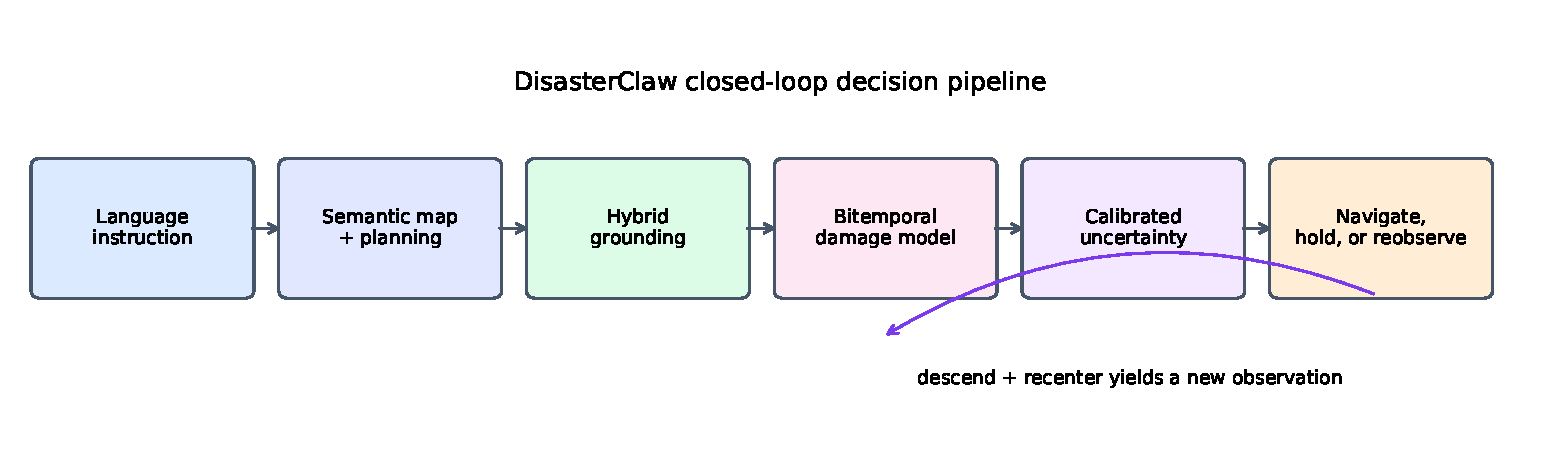
\includegraphics[width=0.96\textwidth]{generated/system_overview.pdf}
  \caption{\ProjectName closes the loop between language-guided navigation,
  bitemporal damage perception, calibrated uncertainty, and a bounded active
  observation action. Planning and mapping provide context; the scientific
  focus is the decision to accept or reacquire visual evidence.}
  \label{fig:overview}
\end{figure*}

\begin{figure}[t]
  \centering
  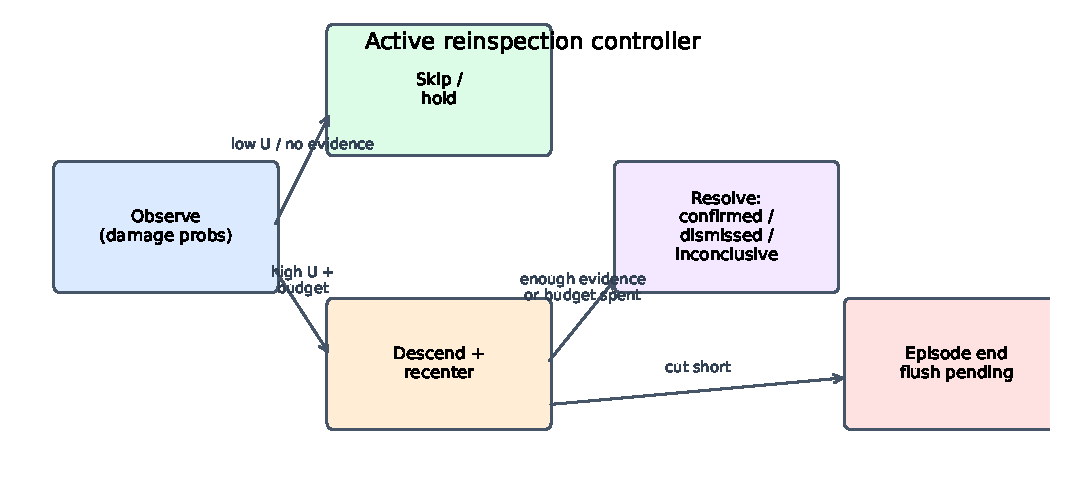
\includegraphics[width=\columnwidth]{generated/recheck_state.pdf}
  \caption{The reinspection controller observes damage probabilities, then
  skips, descends and recenters, or resolves. Open loops are flushed at
  episode end so truncated evidence is not dropped from \(\Delta U\).}
  \label{fig:recheck-state}
\end{figure}

\subsection{Dual-Temporal Damage Perception}
Let \(f_\theta(\cdot)\) be a shared image encoder.
For a building crop, the baseline temporal representation is
\begin{equation}
 z_{\mathrm{cat}} =
 [f_\theta(I^{\mathrm{pre}}), f_\theta(I^{\mathrm{post}}),
 f_\theta(I^{\mathrm{post}})-f_\theta(I^{\mathrm{pre}})] .
\end{equation}
Two prediction heads estimate four-way damage and binary change.
The training objective is
\begin{equation}
 \mathcal{L} = \mathcal{L}_{\mathrm{damage}}
 + \lambda \mathcal{L}_{\mathrm{change}}, \qquad \lambda=0.5 .
\end{equation}

The difference-attention variant applies channel gates to the two temporal features and then gates their difference.
This variant tests whether explicit change-selective channels are preferable to direct concatenation.
Its existing cross-disaster numbers are exploratory because of the historical split risk described above.

\subsection{Probability Calibration}
Given damage logits \(\ell\) and a positive temperature \(T\), calibrated probabilities are
\begin{equation}
 p_k = \frac{\exp(\ell_k/T)}
 {\sum_j \exp(\ell_j/T)} .
\end{equation}
\(T\) is optimized on held-out calibration data by minimizing negative log-likelihood.
We compute normalized predictive entropy
\begin{equation}
 U_t = -\frac{1}{\log K}\sum_{k=1}^{K}p_{t,k}\log p_{t,k},
 \label{eq:entropy}
\end{equation}
where \(K=4\).
Temperature scaling changes confidence but not the argmax class, so improved ECE must not be described as improved recognition accuracy.

\subsection{Uncertainty-Driven Active Reinspection}
The sensing action set is
\(
\calA_{\mathrm{sense}}=\{\texttt{hold},\texttt{descend\_center}\}.
\)
For action \(a\), a geometry-conditioned proxy predicts the entropy after the next observation.
The estimated information gain is
\begin{equation}
 \widehat{\mathrm{IG}}(a)
 = U_t-\widehat{\mathbb{E}}[U_{t+1}\mid a].
\end{equation}
The agent reinspects when it has damage evidence, \(U_t\geq\tau\), a non-hold action has positive gain above a fixed margin, and both local and episode budgets remain.
Otherwise it holds or resolves the current judgment.
Descending shrinks the ground footprint; recentering places the candidate away from the crop boundary.

Each location is quantized into a geographic key.
The controller records its first uncertainty, latest uncertainty, number of attempts, altitude, and terminal status.
Hard limits on descent, minimum altitude, per-location attempts, and total episode attempts prevent an unbounded loop.
If an episode terminates with an open reinspection, the final observation is flushed as \texttt{episode\_end} so that the accounting does not silently discard difficult cases.

\subsection{Supporting Navigation Stack}
The hierarchical semantic planner (HSPM) decomposes multi-landmark instructions, an STMR-style textual map representation exposes nearby semantic cells to the language model, and memory supports retrieval across explored positions.
For building proposals we use an event-disjoint ResNet34 U-Net trained only on pre-disaster tiles from the twelve training events, then convert the predicted mask into boxes by connected components.
Each box is cropped from the paired pre/post patches and scored by the dual-temporal damage classifier above; segmentation and a vision-language fallback remain available for non-building cues.
A weak YOLO detector under the same split is retained only as a localization baseline and rollback path.
Because navigation success stays low and shows no strict-SR improvement attributable to these modules, we treat localization, segmentation, planning, and memory as implementation scaffolding rather than as claimed sources of navigation gains.
